
\documentclass[preprint,12pt]{elsarticle}

\usepackage[spanish]{babel}
\usepackage{amssymb}
\usepackage{graphicx}
\usepackage{lineno}
\usepackage[utf8]{inputenc}
\usepackage{url}
\usepackage{natbib}

\begin{document}
	
	\begin{frontmatter}

		\title{\huge  COMPARATIVA ENTRE INTELIGENCIA DE NEGOCIO (BI) Y ANALITICA DE NEGOCIO(BA) }
		\author{Robles Flores, Anthony Richard	                (2016056192)}
		\author{Estrella Palacios, Katherine Lizbeth			(2015050948)}
		\author{Sosa Bedoya, Sharon					(2016054460)}
		\author{Torres Beltran , Johanna Andrea			(2020067849)}
		\address{Tacna, Perú}
		


%%INICIO abstract
\begin{abstract}
The world is in constant evolution so changes are incorporated into various sectors of society such as: economy, technology, education, health, agriculture, work, etc. 
Therefore this article is focused on the implementation of intelligent solutions in companies to improve their business objectives. 
\\
Business Intelligence and Business Analytics, is not only used by large companies so that small and medium enterprises also see the need to incorporate these solutions to its operation, so the market requires it and consequently increasing profits.
\end{abstract}
%%FIN abstract


\end{frontmatter}

%%INICIO Resumen
\section{Resumen}
El mundo se encuentra en constante evolución por lo cual se incorporan cambios a los diversos sectores de la sociedad como: economía, tecnología, educación, salud, agricultura, trabajo, etc. 
\\
\\
Por lo tanto este articulo esta centrado en lo que respecta a la implementación de soluciones inteligentes en las empresas para mejorar sus objetivos comerciales. 
Business Intelligence y Business Analytics,  no solo es utilizado por las grandes empresa de modo que las pequeñas y medianas empresas también ven la necesidad de incorporar estas soluciones a su funcionamiento, por lo que el mercado así lo requiere y por consecuente el aumento de las ganancias.
%%FIN Resumen


%%INICIO Introducción
\section{Introducción}
El contexto de la sociedad de la información a propiciado tener la necesidad de mejores, más rápido y eficientes 
métodos para extraer y transformar los datos de una organización en información y distribuirla a lo largo de la 
cadena de valor.
\\
\\
En este articulo podremos apreciar los conceptos base acerca de la inteligencia de negocio (Business Intelligence)
 donde responde a esta como una necesidad y podemos entender en una primera aproximación que es una 
evolución de los sistemas de soporte a la decisiones (DSS).
\\

%%FIN Introducción


%%INICIO Marco Teórico
\section{Marco Teórico}

%%----------------------------------------------------------------------------------------------------------------------------------------------------------
	\subsection{\textbf{Inteligencia de Negocios (BI)}}
	Hay que tomar en cuenta que este concepto Business Intelligence es un tema que viene desde octubre de 1958 
por Hans Peter Luhn (Investigador de IBM). Este concepto ha evolucionado aunando diferentes tecnologías, metodologías
 y términos.\cite{referenciarobles1}
\\
\\
Según el glosario de términos de Gartner (2012) se extrae la siguiente definición:
“BI es un proceso interactivo para explorar y analizar información estructurada sobre un área (normalmente almacenada en un “datawarehouse”), para descubrir tendencias o patrones, a partir de los cuales derivar ideas y extraer conclusiones. El proceso de BI incluye la comunicación de los descubrimientos y efectuar los cambios. Las áreas incluyen clientes, proveedores, productos, servicios y competidores.” 
\\
\\
Según Vitt (2002):
“El BI es usado por diferentes usuarios y desarrolladores de software para distinguir un amplio rango de tecnologías, plataformas de software, aplicaciones específicas y procesos. Se utiliza este término desde tres diferentes perspectivas:
	\begin{itemize}
	\item Tomar mejores decisiones rápidamente.
	\item Convertir los datos en información.
	\item Utilizar un método razonable para la gestión empresarial.”   \\
	\end{itemize}

Business Intelligence  es un conjunto de metodologías, aplicaciones, prácticas y capacidades enfocadas a la creación
 y administración de información que permite tomar las mejores decisiones a los usuarios en una organización.

	\subsubsection{\textbf{Componentes de una Arquitectura de BI}}

	Los componentes son:

	\begin{itemize}
	\item Fuentes de información, de las cuales partiremos para alimentar de información el datawarehouse. Las fuentes de información a las que podemos acceder son: de los sistemas operacionales o transaccionales, que incluyen aplicaciones desarrolladas a medida, ERP, CRM, SCM, etc. Sistemas de información departamentales: previsiones, presupuestos, hojas de cálculo, etcétera.
	\item Proceso ETL de extracción, transformación y carga de los datos en el datawarehouse. Antes de almacenar los datos en un datawarehouse, éstos deben ser transformados, limpiados, filtrados y redefinidos. Normalmente, la información que tenemos en los sistemas transaccionales no está preparada para la toma de decisiones.
	\item El propio datawarehouse o almacén de datos, con el Metadata o Diccionario de datos. Se busca almacenar los datos de una forma que maximice su flexibilidad, facilidad de acceso y administración.
	\item El motor OLAP, que nos debe proveer capacidad de cálculo, consultas, funciones de planeamiento, pronóstico y análisis de escenarios en grandes volúmenes de datos.
	\item Las herramientas de visualización, que nos permitirán el análisis y la navegación a través de los mismos.

	\end{itemize}

\begin{figure}[htb]
	\begin{center}
		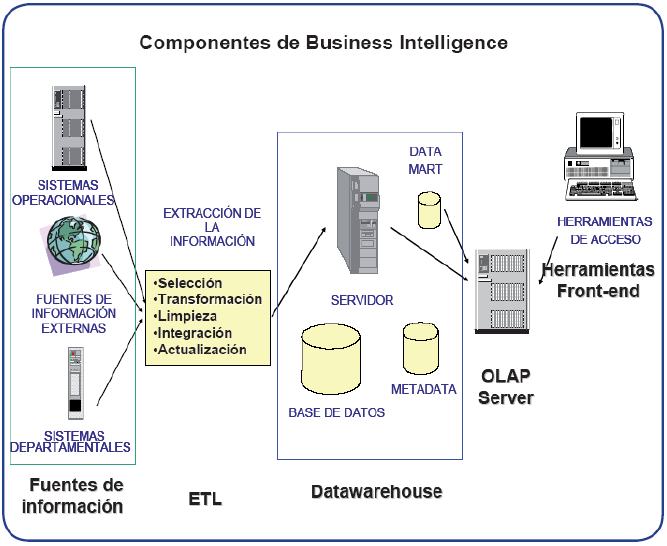
\includegraphics[width=14cm]{./IMAGENES/componentes} 
		\caption{Componentes de Business Intelligence}
	\end{center}
\end{figure}

%%****

\subsubsection{\textbf{El ciclo de la Inteligencia de Negocios}}

La Inteligencia de Negocios en una plataforma de administración del desempeño que representa al ciclo en el que las empresas establecen sus objetivos, analizan sus progresos, reflexionan, actúan, miden su éxito y empiezan una nueva fase. \\ \\Su ciclo se compone de cuatro etapas a saber: Análisis, reflexión, acción y medición. (Peña, 2006).

\begin{figure}[htb]
	\begin{center}
		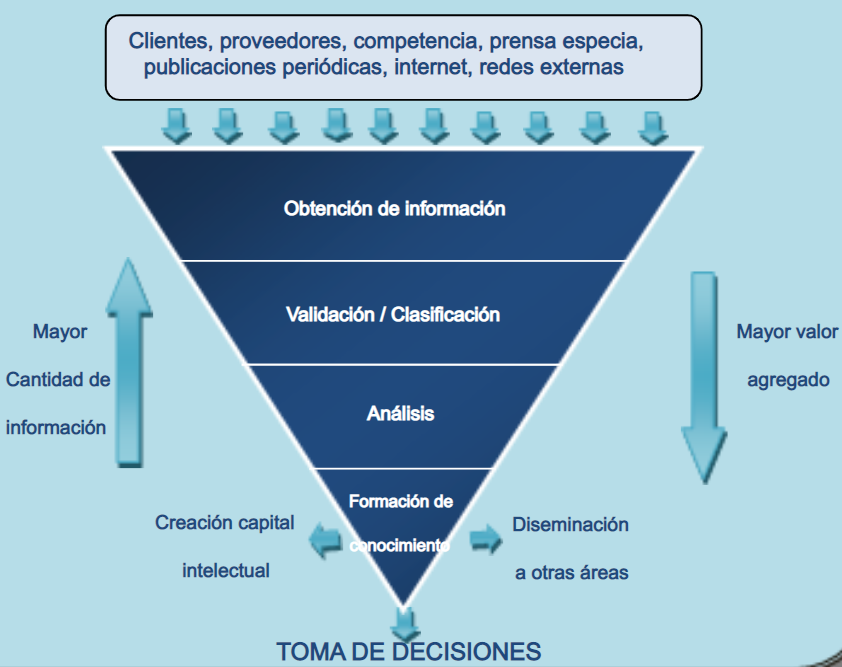
\includegraphics[width=12cm]{./IMAGENES/ciclo_BI} 
		\caption{Ciclo de Inteligencia de Negocios}
	\end{center}
\end{figure}

%%****
	\subsubsection{\textbf{Beneficios de un sistema de Inteligencia de Negocio (BI)}}
	La implantación de estos sistemas de información proporciona diversos beneficios entre los que podemos destacar:

	\begin{itemize}
	\item Crear un circulo virtuoso de la información (Donde los datos se transforman en información que permitirá 
		generar conocimiento para una toma de decisiones que se traducirán en mejores resultados y que 
		generarán nuevos datos).
	\item Permite una visión única, conformada, histórica, persistente y de calidad de toda la información. 
	\item Crear y manejar métricas, indicadores claves de rendimiento, e indicadores claves de meta fundamentales 
		para la empresa.
	\item Aportar información actualizada tanto a nivel agregado como en detalle.
	\item Reducir el diferencial de orientación de negocio entre el departamento de TI y la organización. 
	\item Mejorar comprensión y documentación de los sistemas de información en el contexto de una organización.
	\item Mejorar la competitividad de la organización como resultado de ser capaces de diferenciar lo relevante sobre 
		lo superfluo, acceder más rápido a la información, tener mayor agilidad en la toma de decisiones.
	\end{itemize}
%%****
	\subsubsection{\textbf{La necesidad de la Inteligencia de Negocio}}
	Existen situaciones en las que la implantación de un sistema Business Intelligence  resulta adecuada. Podríamos destacar 
	entre las que existen son:

	\begin{itemize}
	\item La toma de decisiones se realiza de forma intuitiva en la organización resultados y que generarán nuevos datos).
	\item Identificación de problema de calidad de información
	\item Uso de Excel como repositorios de información corporativos o de usuario o conocido como el Excel Caos.
	\item Necesidad de cruzar información de forma ágil entre departamentos.
	\item Evitar sirios de información.
	\item Las campañas de marketing no son efectivas por la información base usada. 
	\item Existe demasiada información en la organización para ser analizada de la forma habitual (se alcanzó la masa crítica de datos).
	\end{itemize}
%%****
	\subsubsection{\textbf{Estrategia de Business Intelligence}}
	Desplegar un proyecto de inteligencia de negocio en una organización no es un proceso sencillo. Las buenas practicas dicen 
	que para llegar a un buen puerto, es necesario tener una estrategia de inteligencia de negocio que coordine de forma efectiva 
	las tecnologías, el uso, los procesos de madurez.\cite{referenciarobles2}
%%****
	\subsubsection{\textbf{Ausencia de una estrategia de BI}}
	Es posible detectar que no existe estrategia definida a través de los siguientes puntos:

	\begin{itemize}
	\item Los usuarios identifican al departamento de TI como el origen de problemas de inteligencia de negocios.
	\item La dirección considera que la inteligencia de negocios es otro centro de coste.
	\item El departamento de TI continúa preguntando a los usuarios finales sobre las necesidades de los informes.
	\item El sistema de BI esta soportado por help desk.
	\item No hay diferencia entre BI y gestión de rendimiento.
	\item No es posible medir el uso de inteligencia de negocio.
	\item Se considera que la estrategia para el datawarehouse es la misma que para que el sistema de inteligencia de negocio.

	\item No hay un plan para desarrollar, contratar, retener y aumentar el equipo de BI.
	\item No se conoce si la empresa tiene una estrategia para el BI.
	\item No existe un responsable funcional.
	\item No existe un centro de competencia.
	\item No hay un plan de formación real y consistente del uso de las herramientas.
	\item Los usuarios creen que la información del datawarehouse no es correcta.
	\end{itemize}


%%****
	\subsubsection{\textbf{Desarrollo de una estrategia de BI}}
	Desarrollar una estrategia de negocio es un proceso a largo plazo que incluyen múltiples actividades donde podríamos destacar:

	\begin{itemize}
	\item Crear un centro de competencia de BI. Tiene el objetivo de armonizar conocimientos en tecnologías, metodologías, estrategias 
	con la presencia de un sponsor a nivel ejecutivo y analistas de negocio implicados y que tengan responsabilidades compartidas en 
	éxitos y fracasos.
	\item Establecer estándares de BI en la organización para racionalizar tanto las tecnologías existentes como las futuras adquisiciones.
	\item Desarrollar un Framework de métricas a nivel empresarial.
	\item Revisar y evaluar el portafolio actual de soluciones en un contexto de riesgo/recompensa.
	\item Aprender de los éxitos y fracasos de otras empresas revisando casos de estudio y consultar a las empresas del sector para 
	determinar que a funcionado y que no.
	\item Poner atención a las necesidades que requieren BI en la organización porque se acostumbra a satisfacer a los usuarios o 
	departamentos que gritan mas fuerte. Es decir, dar más atención a todas las áreas en atención en solución BI.
	
	\end{itemize}



%%-----------------------------------------------------------------------------
	\subsection{\textbf{Analítica de Negocios (BA) }}
	Business Analytics son un conjunto de tecnologías que ayudan a los usuarios a analizar grandes datos empresariales para tomar decisiones mejores y más efectivas. \\\\
Es una colección de habilidades, tecnologías, aplicaciones y prácticas para la investigación continua y repetitiva de los datos, y así poder explicar el desempeño empresarial histórico, actual y futuro\cite{referenciasosa1}.\\
\\Al estudiar estos datos, las empresas pueden responder preguntas como“¿Qué está pasando?”, “¿Por qué está sucediendo?” Y “¿Qué va a pasar?”\cite{referenciasosa3}, también determinar los mejores modelos y enfoques analíticos, descubriendo las oportunidades actuales y tendencias futuras acerca de los clientes en relacón con su producto/servicio, y así presentar estas soluciones, a los usuarios empresariales, que permitirán a la organización alcanzar sus objetivos estratégicos.\\
Schnierderjans et al.(2014) en su libro resumieron que el BA incluye los mismos procedimientos que en la analítica simple, pero tiene el requisito adicional de que el resultado del análisis analítico debe tener un impacto medible en el rendimiento de la empresa. \cite{referenciasosa2} \\
\\Simplemente, los análisis convierten los datos en información útil para la empresa.

	\subsubsection{\textbf{Tipos de Analítica }}
	\begin{itemize}
	\item{\textbf{1. Análisis descriptivo:}}se encargar de realizar un seguimiento en base a los indicadores  clave de rendimiento 			para comprender el estado actual de una empresa. 		
	\item {\textbf{2. Análisis  predictivo:}}se centra en analizar los datos de tendencia con el proposito de recomendar acciones que 
	den solución a situaciones iguales al futuro.
	\item {\textbf{3. Análisis prescriptivo:}}Utiliza la implementación de tendencias estadísticas para determinar la probabiliad de 			eventos futuros. 
	\end{itemize}

	\subsubsection{\textbf{BA Framework }}
El marco general de BA incluye cuatro capas: capa de datos, capa de análisis, capa de información / visualización y capa de acceso.
Estas capas se analizan a continuación\cite{referenciasosa1}: 
\begin{figure}[htb]
	\begin{center}
		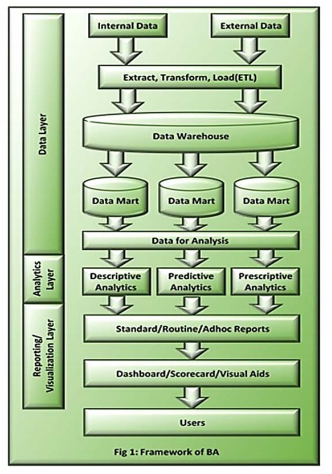
\includegraphics[height=10cm]{./IMAGENES/BAFramework} 
		\caption{Framework de BA}
	\end{center}
\end{figure}

	\begin{itemize}
	\item \textbf{Capa de datos:} se recopilan los datos de fuentes internas y externas. Las fuentes de datos internas incluyen la base de datos operativa de la organización que almacena las transacciones diarias,y las externas incluyen proveedores, clientes, competidores, agencias gubernamentales, Internet, etc. Los datos recopilados se almacenan en un almacén de datos y luego se analizan para tomar decisiones.
	Algunas herramientas utilizadas en la capa de datos se encuentran:
		\begin{itemize}
		\item  Data Warehouse: Es una colección de información corporativa derivada directamente de los sistemas operacionales (fuentes internas) y algunas fuentes de datos externas. El almacén de datos es una copia de los datos de las transacciones estructurada específicamente para la consulta y el análisis. 
		\item Data mart: también conocidos como almacenes de datos localizados, son pequeños almacenes de datos, generalmente creados por varios departamentos o departamentos para proporcionar sus propias actividades de soporte de decisiones.
		\item Minería de datos: la minería de datos es el proceso de explorar y analizar grandes cantidades de datos a través de medios semiautomáticos o automáticos para descubrir patrones y reglas importantes.
		\end{itemize}

	\item \textbf{Capa de Análisis:} En esta capa, los datos del Data Warehouse/DataMart se analizan mediante análisis descriptivos, predictivos y preceptivos.
		\begin{itemize}
		\item Minería de datos: la minería de datos es el proceso de explorar y analizar grandes cantidades de datos a través de medios semiautomáticos o automáticos para descubrir patrones y reglas importantes. Es la técnica que incluye la ciencia de la gestión, los modelos y métodos estadísticos, matemáticos y financieros que determinan las relaciones vitales entre variables en datos históricos, analizan datos o hacen pronósticos.
		\item Análisis de datos multidimensionales: conocido como procesamiento analítico en línea (OLAP), permite a los gerentes, ejecutivos y analistas obtener una comprensión más profunda de los datos al acceder a varias vistas de información multidimensional de manera rápida, confiable y colaborativa. Permite a los analistas de negocios utilizar estos datos, cambiando las relaciones para obtener una vista más detallada de la información de la empresa. \\El análisis multidimensional permite a los usuarios ver los mismos datos de diferentes maneras usando múltiples dimensiones, como por región, producto, costo, precio.
		\end{itemize}

		\item \textbf{Capa de Reportes y Visualización:} En esta capa se encuentran varias herramientas para poder visualizar la información analizada:
		\begin{itemize}
		\item Dashboard: son herramientas para visualizar datos comerciales importantes que se muestran en forma de indicadores gráficos, cuadros y tablas. \\Los paneles digitales ofrecen a los usuarios una vista gráfica avanzada de los procesos comerciales, que se puede subdividir para encontrar información más detallada sobre procesos comerciales específicos.
		\item Balanced Scorecards: El concepto de los Cuadros de Mando Integral (BSC) fue presentado por Kaplan. Se trata de informes estructurados semiestándar, apoyados por instrumentos y técnicas de diseño, que pueden ser utilizados por los administradores para hacer un seguimiento de la ejecución de las actividades por el personal que está bajo su control y para vigilar las consecuencias que se derivan de esas acciones. 
\begin{figure}[htb]
	\begin{center}
		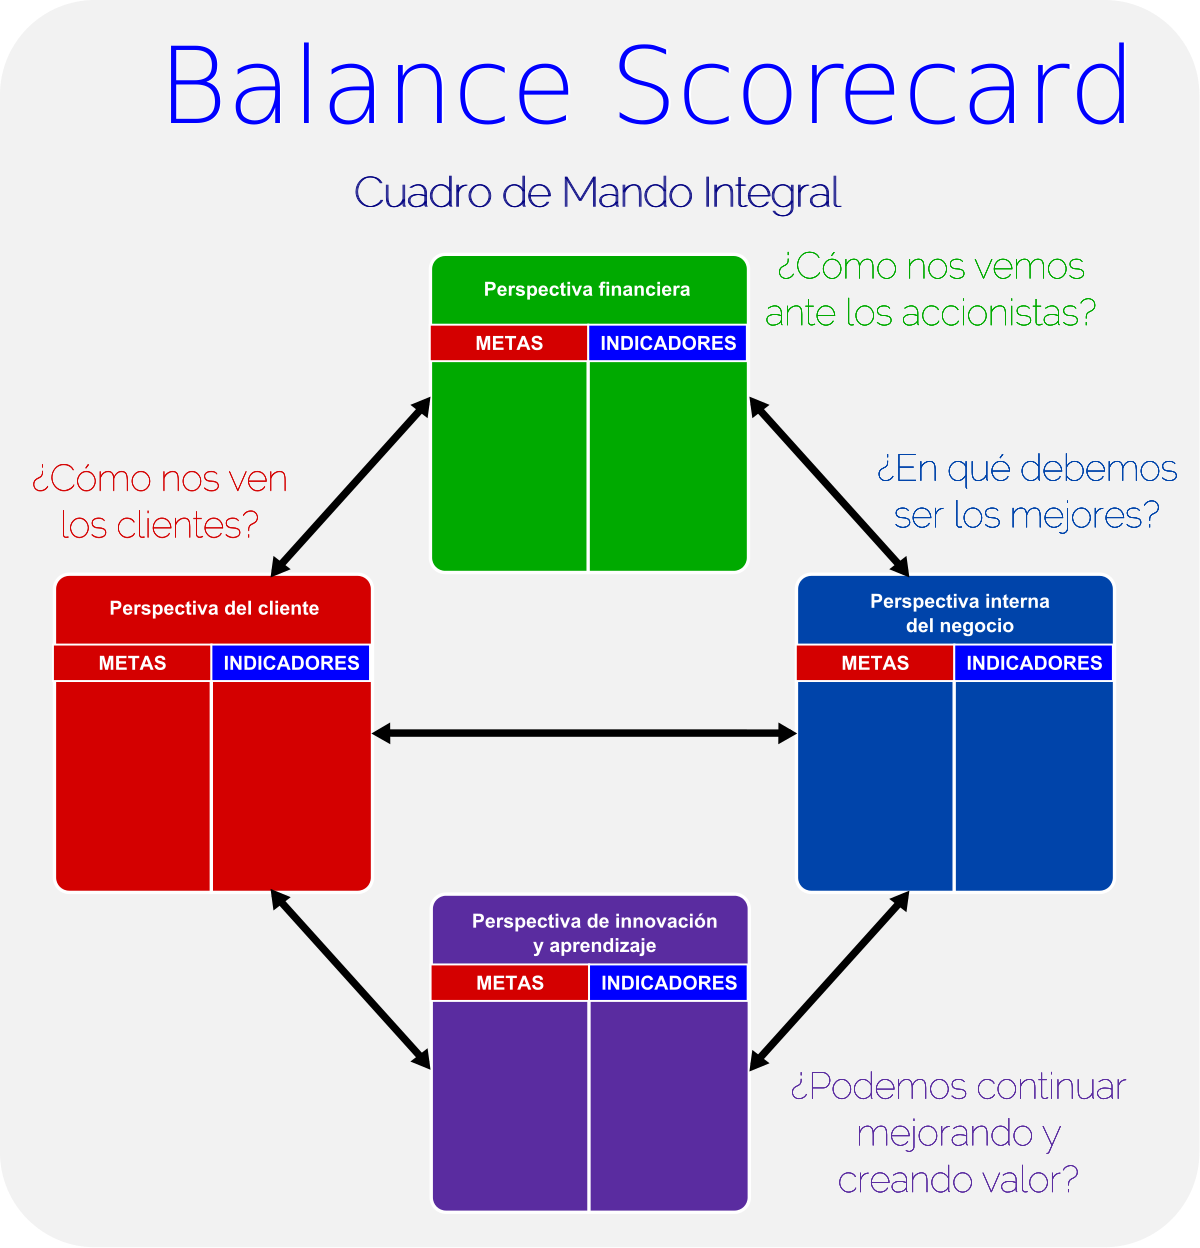
\includegraphics[width=8cm]{./IMAGENES/BalanceScorecard} 
		\caption{BalanceScorecard por Kaplan}
	\end{center}
\end{figure}


		\item Informes: Son los documentos escritos relativos a la situación y pueden ser creados por los usuarios finales mediante el suministro de datos de parámetros. Los resultados de los informes preejecutados se almacenan en caché para permitir una visualización interactiva y de alto rendimiento de estos informes.
		\item Informes ad hoc: A diferencia de los informes estándar, que están predefinidos y se procesan de forma rutinaria, los informes ad hoc se generan cuando surge la necesidad. Permiten a los usuarios producir sus propios informes personalizados sin depender del equipo de TI.
		\end{itemize}

	\end{itemize}
%%-----------------------------------------------------------------------------
	

%%----------------------------------------------------------------------------------------------------------------------------------------------------------
%%FIN Marco Teórico

%COMPRACION
\section{Comparación entre Inteligencia de Negocios (BI) y Analítica de Negocios (BA)}
A continuacion se muestra la comparación entre Inteligencia de Negocios y Analítica de Negocios:
	
	\begin{itemize}

	\item{\textbf{1.}} La inteligencia de negocios utiliza datos del pasado y actuales, mientras que la analítica de negocios utiliza 			datos del pasado para extraer información y ejecutrar las operaciones comerciales que suplen las necesidades del cliente y por 		consecuente aumentan la productividad.
	\item{\textbf{2.}} La inteligencia de negocios se enfoca principalmente en informar los datos analizados, mientras que la analítica 	de negocios se centra en múltiples herramientas que realizan diferentes aplicaciones operativas utilizando diferentes 				herramientas.
	\item{\textbf{3.}} La inteligencia de negocios casi se incluye en la analítica de negocios, donde la analítica de negocios contiene 		inteligencia de negocios, en el almacenamiento de datos, gestión de información, aplicaciones empresariales y gobierno, y por 			último el cumplimiento de riesgos y seguridad.
	\item{\textbf{4.}} La inteligencia de negocios es la forma de analizar los datos existentes, mientras que la analítica de negocios 		tendrá informes de inteligencia de negocios que actúan como entradas para que los análisis procesen la información extraída de 		una manera más sofisticada para visualizar los datos analizados.
	\item{\textbf{5.}} La inteligencia de negocios utiliza análisis estadísticos, análisis predictivos y modelos predictivos para 				establecer las tendencias actuales y descubrir las razones de los resultados o acontecimientos actuales, mientras que la 			analítica de negocios no tiene control sobre las grandes cantidades de datos para poder recuperar, analizar, informar y publicar 		datos.
	\item{\textbf{6.}} La inteligencia de negocios consiste más en paneles de interfaz de usuario para poder llevar a cabo el análisis 		y las operaciones, mientras que la analítica de negocios tiene muchas herramientas para trabajar y eso también necesita algunos 		conomientos de aplicaciones de software para llevar a cabo las tareas a realizar.
	\item{\textbf{7.}} La inteligencia de negocios brinda información sobre los datos en sí mismos en lugar de realizar 				transformaciones o conversiones adicionales para brindar información sobre los datos y, por otro lado, la analítica de negocios 			implica la forma de resolver problemas al habilitar las tecnologías al transformar la forma cruda de datos en una forma significativa 	para transmitir la solución de una manera fácil.
	\end{itemize}

%CONCLUSIONES
\section{Conclusiones}
\subsection{Conclusión }	
%%****
Como conclusion acerca de Business Intelligence es que nos sirve para poderdar soluciones a ciertas igconitas a la organizacion que 
podria pasar por un momento donde se carece de una estrategia de BI.
Sobre el ¿Qué esta pasando?¿Qué pasa ahora?¿Porqué pasó?¿Que pasará? y asi mismo pueda darse una solución a la problematica 
existente dentro de sus áreas.\\\\
Durante la última década, la calidad de BA ha mejorado significativamente, permitiendo a los gerentes utilizar las cantidades masivas de datos almacenados en bases de datos operacionales y almacenes de datos para comprender mejor el negocio y predecir posibles amenazas para la organización.




%RECOMENDACIONES
\section{Recomendaciones}	
CONTENIDO






	
	\newpage
	\bibliographystyle{apalike}
	\bibliography{BIBLIOGRAFIA}	
%\citep{referenciarobles2}  


% https://revistas.udistrital.edu.co/index.php/tia/article/view/4639/7094
% http://revistas.unitru.edu.pe/index.php/PGM/article/view/193/199
% http://www.spentamexico.org/v4-n2/4(2)%2016-52.pdf          ---> PAGINA 18


\end{document}

